\documentclass[11pt,a4paper]{article}
\usepackage[margin=25mm]{geometry}
\usepackage{amsmath,amssymb,booktabs,microtype,tikz}
\usepackage[hidelinks]{hyperref}
\usepackage{xurl}
\usepackage[section]{placeins}
\title{Digital-Twin-Guided Predictive Autoscaling:\\A Pilot Study of Workload and Latency-Model Calibration}
\author{Shehryar Faisal}
\date{October 2026}
\begin{document}\maketitle
\begin{abstract}
Workload uncertainty and errors in translating demand into application latency are distinct sources of risk in predictive autoscaling. We implement a service-response Digital Twin with separate online residual corrections for demand and tail-latency estimates, then evaluate its limitations in a reproducible pilot study. The work first preserves and validates a published Prophet--LSTM baseline. On additional held-out forecasts, adaptive upper bounds attain workload coverage close to a nominal 90\% without implying request-level SLO guarantees. A measured CPU-service profile initializes a monotone latency Twin. We then execute 350 trials using a separate queueing plant and 15 Kubernetes controller runs, including component ablations, burst traffic and a service-cost shift.

In the live study, dual calibration has mean request-violation rate 10.40\%, versus 39.67\% for the point-Twin policy, and uses 7.65 versus 6.54 sampled pod-minutes. Dual calibration meets the 99\% request SLO in 1 of three runs. These are finite, workload-specific observations rather than a general superiority claim. The results characterize the cost of conservative corrections and the limits imposed by startup, drift and model support. No formal end-to-end latency guarantee is asserted.\end{abstract}


\section{Introduction}
Kubernetes autoscaling must turn incomplete demand measurements into resource decisions before new capacity becomes ready. CPU-based Horizontal Pod Autoscaling (HPA) is an operational reference, while KEDA connects external signals to Kubernetes scaling \cite{k8s,keda}. Forecasting alone does not determine how many replicas satisfy an application latency objective: the workload-to-performance mapping can also change with request cost, resource throttling and readiness.

Our starting point is the released Prophet--LSTM approach of Guruge and Priyadarshana \cite{guruge}. We preserve its implementation and reproduce its calculations before introducing a separate causal evaluation. This distinction matters because timestamp alignment and test-dependent transformations change the meaning of a reported forecasting error. We subsequently study control uncertainty using a separate, instrumented CPU service; the authors' application and original results are not modified.

This paper makes a bounded empirical contribution. It provides an auditable baseline validation, implements a forecaster-independent controller with two residual-calibration channels, and evaluates the channels separately and jointly. The Digital Twin is a measured service-response surrogate, not a replica of the entire cluster. We do not claim that conformal autoscaling, latency-aware scaling or Kubernetes Twins are new. The specific question is whether calibrating the Twin's mapping error adds useful protection beyond calibrating demand, and what resource cost accompanies that protection in a small controlled deployment.

We examine three questions: (RQ1) how do adaptive workload bounds behave on held-out historical forecasts; (RQ2) how do the two correction channels affect measured latency and allocation; and (RQ3) how sensitive is the controller to service drift, observation delay and startup mismatch? The evidence levels are separated: historical forecasting, simulation and Kubernetes measurements answer different parts of these questions.

\section{Related Work}
Prophet models configurable trend and seasonal structure \cite{prophet}; LSTM introduces gated recurrent memory \cite{lstm}. Their use in the reference hybrid assigns trend/seasonality to Prophet and residual prediction to an LSTM \cite{guruge}. Our faithful reproduction targets the hybrid results, not every comparator in the original article.

Adaptive conformal inference adjusts a calibration level using observed misses \cite{aci}; later work addresses adaptation under arbitrary distribution shifts \cite{online}. Our implementation uses a finite rolling score window, clipped levels and nonnegative corrections. These engineering choices are explicitly evaluated and do not inherit the unmodified algorithms' theoretical guarantees. Forecast-bound coverage must also be distinguished from request-latency compliance.

BACC version 2 combines forecast calibration, measured service-risk profiling and budget pacing, and evaluates both latency and CPU SLOs \cite{bacc}. Its October 2026 revision supersedes a CPU-only comparison with version 1; latency-aware calibration is therefore not our novelty claim. BACC refits a monotone violation-risk profile. We instead keep a fitted effective-P99 surrogate frozen and adapt a separate residual margin, studying this choice through ablation rather than claiming it superior to BACC.

KARMA constructs a cluster-trace Twin for simulation-based multi-agent training and transfers policies to Kubernetes \cite{karma}. SLO-Scaler describes Bayesian workload/tail-latency prediction with dependency-aware decisions \cite{sloscaler}. InferScale combines early demand signals, SLO-state control and readiness-sensitive execution \cite{inferscale}. These works establish substantial overlap with the general proposal. We do not reproduce their full systems or compare our performance with their reported numbers; the present study is a small, transparent calibration experiment rather than a state-of-the-art ranking.

\section{Problem and Baseline Validation}
Let $y_t$ denote workload in consistent model units, $p_t$ a frozen Prophet estimate and $r_t=y_t-p_t$ a residual. A causal one-minute hybrid predicts
\begin{equation}\widehat y_{t\mid t-1}=p_t+f_\theta(r_{t-1}).\end{equation}
Training-only transformations are applied and inverted where appropriate. The scored observation at $t$ is excluded from its own input. Later forecasts may use earlier observed test counts: this is rolling one-step evaluation, not recursive multi-step prediction.

The official supplied NASA and WorldCup98 files contain 81,396 and 125,300 observed minute rows, respectively. Their chronological 70/30 partitions contain 56,977/24,419 and 87,710/37,590 train/test rows. They omit 7,884 and ten calendar minutes. The corrected evaluation removes nonconsecutive source/target pairs without asserting missing traffic is zero; 24,390 NASA and 37,590 WorldCup targets remain. Raw-trace reconstruction is not repeated.

The released main notebooks use linear Prophet growth for NASA and flat growth for WorldCup; changepoint prior 5.1; seasonality prior 30; weekly/daily Fourier orders 20/50; and no yearly seasonality. Two 50-unit LSTM layers and a linear output use look-back one, Adam/MSE, batch 16, a 20-epoch cap, validation fraction 0.2 and patience-five early stopping with restored best weights. The article prints 50 epochs. Four faithful fits (two per dataset) stop after six epochs and restore epoch-one weights. The executed CPU environment uses Python 3.12.14, TensorFlow 2.17, Keras 3.4.1 and Prophet 1.1.5 on an Intel i7-1255U.

The released combination assigns a next-row residual prediction to the current row and fills its final missing prediction with observed truth. NASA residual scaling and WorldCup count scaling include test data. These behaviours are retained in the faithful runs. A separate corrected implementation fixes alignment, removes the truth fallback and fits transforms on the early neural fitting prefix. Prophet still fits the entire outer training period, making neural validation conditional on that fitted Prophet; the outer test is outside fitting. Full random-state seeding to 42 and gap filtering are additional changes, so this validation is not a one-factor ablation.


\begin{table}[htbp]\centering\small\setlength{\tabcolsep}{4pt}
\caption{Baseline forecast RMSE. Released means use the original full test; causal NASA omits 29 gap targets. WorldCup values use the common author display scale only after causal training.}\label{tab:baseline}
\begin{tabular}{lrrr}\toprule
Dataset & Published RMSE & Released mean & Causal RMSE\\\midrule
NASA & 7.990 & 8.02163 & 14.2902\\
WorldCup & 0.003358 & 0.00337950 & 0.00388174\\
\bottomrule\end{tabular}\end{table}


On NASA common eligible targets, the released mean RMSE is 8.01251. WorldCup causal raw-count RMSE is 890.5685, compared with persistence at 762.7463; NASA persistence is 16.3871. Higher causal error changes the interpretation of the released scoring but cannot be assigned to one isolated correction. Original outputs remain preserved.

An earlier integration check connected the authors' Java 21/Spring Boot 3.4.2 application and external forecasting scaler to KEDA 2.18, Prometheus 2.55.1 and local K3s. The scaler logic was preserved while regenerating compatible gRPC bindings. Stable, increasing, spike and decreasing traffic scenarios produced 6,870 measured requests per controller in scheduling-validated runs. Both forecast KEDA and CPU HPA had zero HTTP failures and zero observations above 500 ms. Forecast scaling held three replicas, whereas HPA moved from one to three; sampled allocation was 23.286 versus 13.778 pod-minutes. These short, unreplicated integration sequences did not reach a useful overload boundary. Diagnostic timing-invalid and aborted attempts remain archived. They establish baseline actuation, not evidence that the proposed uncertainty corrections improve performance; the new stress experiments below use a separate CPU service.

For control, let $\ell_i$ be measured client latency. An observation complies only when HTTP status is 200 and $\ell_i\leq500$ ms. The experimental request SLO is at least 99\% compliance:
\begin{equation}v=\frac{\sum_i\mathbf1\{\mathrm{status}_i\ne200\;\lor\;\ell_i>500\mathrm{\ ms}\}}{N}\leq0.01.\label{eq:slo}\end{equation}
Forecast/model coverage targets below are 90\%, not 99\%. They concern prediction events and cannot be substituted for Equation~\ref{eq:slo}. Allocation is measured by sampled desired-replica pod-minutes, including pending capacity and idle drain intervals; it excludes control-plane/external-controller overhead and is not monetary cost.

\section{Implemented Twin and Controller}
\subsection{Measured Service-Response Twin}
The new controlled service performs PBKDF2 CPU work behind one processing semaphore per pod. Each pod requests 250m CPU/96Mi memory and is limited to 500m/192Mi. Readiness includes an explicit five-second startup delay. A queue wait beyond two seconds returns HTTP 429; clients time out after three seconds. This is a separate benchmark service, not a replacement for the author application or a real inference model.

We profile one replica in 30 chronological cycles. The first 18 use rates $\{5,8,11,14,17,20\}$ requests/s crossed with work multipliers $\{0.75,1,1.25\}$; the last 12 use rates $\{6,9,12,15,18,21\}$ crossed with $\{0.8,1.2\}$. Each cycle offers five seconds of traffic and then reserves three seconds for drainage. The first partition fits the Twin and the second initializes its residual correction. This chronological design is not an exchangeable random split.

For rate $\lambda$, ready replicas $n$ and measured median CPU milliseconds $c$, the Twin input is $x=\lambda c/n$. Isotonic regression fits a nondecreasing effective-P99 response $g(x)$ to the 18 fitting blocks. Effective latency equals measured latency for successful requests and at least 2,000 ms for failures; the penalty prevents fast rejections from making an overloaded service look healthy. Reported SLO violations and client quantiles still use actual status and measured latency. The fitted curve is frozen. A candidate above the profiled $x$ range is rejected, rather than treating clipped extrapolation as evidence of safety. The current CPU-cost estimate is an EWMA with weight 0.5 on the latest completed-cycle median.

\subsection{Separate Residual Corrections}
The short-horizon demand predictor uses the mean of the last three observed rates plus a nonnegative recent trend. It is floored by current rate. It is deliberately lightweight and independent of the historical hybrid; these tests evaluate the control wrapper rather than neural forecasting superiority. Nominal five-RPS prehistory initializes the live controller; those repeated initial values are assumptions, not twelve measured calibration cycles.

Let $h=2$ be the nominal planning horizon in control cycles. A demand score is the realized maximum over the next $h$ cycles minus the issued point maximum. A plan is scored only after its full horizon has completed. Mapping scores compare observed effective-P99 with the frozen Twin at the realized rate and start-of-cycle ready count, using the prior CPU estimate. Mapping coverage is therefore conditional on realized state; it is not an ex-ante joint latency guarantee.

For either channel, retain the last $m\leq40$ signed scores. With target $\alpha_0=0.1$, choose
\begin{align}
j_t&=\min\{m,\max(1,\lceil(m+1)(1-\alpha_t)\rceil)\},\\
q_t&=\max\{0,s_{(j_t)}\},\\
\alpha_{t+1}&=\operatorname{clip}_{[0.025,0.4]}\bigl(\alpha_t+0.01[\alpha_0-\mathbf1\{s_t>q_t\}]\bigr).
\end{align}
Scores enter only after their outcomes are observed. Small-sample ranks are capped at the largest observed score; negative corrections are clipped to zero. This is an ACI-style engineering rule, not a claim of exact finite-sample or arbitrary-drift coverage. In particular, the clipping changes the usual long-run argument.

\subsection{Replica Selection and Execution}
Let $q^D_t$ and $q^G_t$ be the demand and Twin margins. The policy enumerates $n\in\{1,\ldots,6\}$ and selects the smallest supported candidate satisfying
\begin{equation}g\!\left(\frac{(\widehat\lambda_t+q^D_t)c_t}{n}\right)+q^G_t\leq500\mathrm{\ ms}.\label{eq:decision}\end{equation}
If no candidate is supported and feasible, it requests the maximum and records infeasibility. This fallback does not make the constraint true. Scale-ups may proceed immediately; scale-down requires three consecutive lower recommendations and no pending ready deficit. The $h=2$ horizon covers nominal readiness plus the next decision interval; a simulation ablation uses $h=1$. No adaptive startup estimator or global optimality claim is made.

\begin{figure}[htbp]\centering
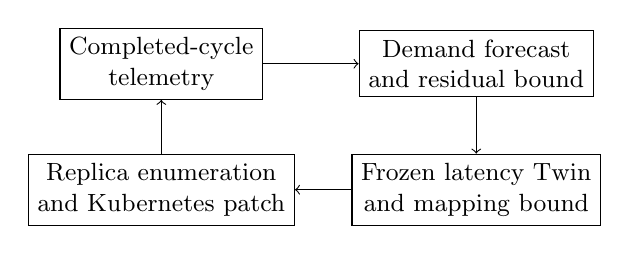
\begin{tikzpicture}[font=\small]
\node[draw,align=center] (m) at (0,0) {Completed-cycle\\telemetry};
\node[draw,align=center] (d) at (4,0) {Demand forecast\\and residual bound};
\node[draw,align=center] (g) at (4,-1.6) {Frozen latency Twin\\and mapping bound};
\node[draw,align=center] (a) at (0,-1.6) {Replica enumeration\\and Kubernetes patch};
\draw[->] (m)--(d);\draw[->] (d)--(g);\draw[->] (g)--(a);\draw[->] (a)--(m);
\end{tikzpicture}
\caption{Implemented feedback loop. Outcome updates precede the next forecast; future workload specifications are not controller inputs.}\label{fig:architecture}\end{figure}

\section{Experimental Design}
\subsection{Historical Workload-Bound Evaluation}
We reuse saved causal forecasts without retraining predictor weights. The first 20\% of their eligible outer-test targets form a new calibration prefix: 4,878 NASA and 7,518 WorldCup targets. The remaining 19,512 and 30,072 targets provide a separate rolling evaluation. Static split calibration uses the prefix's 90\% upper-error quantile. Adaptive calibration starts from its last 40 scores and updates only after each evaluation outcome. Bound margins are measured in physical request counts, with identical issued point forecasts for both methods. These are temporally dependent trace results, not independent-sample coverage certification.

\subsection{Independent Simulation Plant}
The simulator never calls $g$ to generate latency labels. It dispatches Poisson arrivals to the earliest free ready server, using independent lognormal CPU work with log-scale standard deviation 0.3 and a baseline fitted from measured median CPU time. Each ready server supplies 0.5 CPU core. Queue admission and client timeout limits are represented separately. Removed servers drain queued outcomes; the plant is intentionally simpler than Kubernetes CFS and networking.

Each rollout has 64 eight-second cycles. Ten fixed seeds are shared across policies in five regimes: smooth demand; periodic bursts; an additional 1.8-fold service-cost shift halfway through; startup delay increased from eight to 24 seconds; and one-cycle delay of demand/latency/CPU observations while replica state remains current. Seven policies give 350 rollouts. They are point Twin, demand-only calibration, mapping-only calibration, both channels, both channels with $h=1$, a same-cadence CPU-reactive proxy, and static six replicas. The proxy is not native HPA. CPU feedback counts only service executed by the current time; latency feedback uses completed outcomes and explicitly censored outstanding ages. All policies see the same generated arrivals and service requirements within each paired seed/regime.

\subsection{Kubernetes Protocol and Ablations}
The live cluster is K3s v1.33.6+k3s1/containerd 2.1.5 in Ubuntu WSL2 on the same local CPU host. A loopback-only API proxy lets the experimental controller patch its separate deployment. HPA uses native metrics-server CPU observations, a 70\% CPU-request target, replica bounds one to six, no scale-up stabilization and a 24-second scale-down window. Native HPA reconciliation differs from the approximately eight-second external loop; this is an operational reference rather than a timing-matched algorithm comparison.

Five policies (point, demand-only, mapping-only, dual calibration and CPU HPA) each run under seeds 101, 202 and 303. Per-seed policy order is shuffled deterministically. Each trial resets to one ready replica and discards two warm-up cycles. The 16 active-cycle rates are
\begin{center}\small 5, 5, 5, 5, 10, 15, 20, 25, 45, 45, 15, 10, 25, 30, 15, 5.\end{center}
The last four cycles raise work cost from 1 to 1.8; the controller receives no future rate or work schedule. Each cycle offers five seconds of seeded, jittered request slots and a fixed three-second drain, yielding 1,400 requests per trial and 21,000 over 15 trials. Connections are not kept alive, reducing persistent service-routing imbalance. Replica state is sampled at cycle start. The fixed drain makes these controlled batch cycles, not continuous production traffic.

The point/demand-only/mapping-only/dual policies form a two-factor component ablation with identical underlying predictor, Twin, bounds and scale-down guard. All runs are retained. We check request counts, status-derived violations, quantiles, scheduling delay and cycle duration before aggregation. Live results use means and ranges across three executions; simulator differences use paired seed means with descriptive 5,000-resample bootstrap intervals. These intervals characterize the chosen synthetic seeds, not a population of production clusters. Source, protocol and baseline evidence are preserved separately.

\section{Results}
\subsection{Workload Calibration}


\begin{table}[htbp]\centering\small\setlength{\tabcolsep}{4pt}
\caption{Held-out workload upper-bound coverage; nominal target 90\%. Margins are request counts, not interval widths or latency bounds.}\label{tab:coverage}
\begin{tabular}{lrrrrr}\toprule
Trace & Point (\%) & Static (\%) & Adaptive (\%) & Static $q$ & Adaptive $q$\\\midrule
NASA-HTTP & 57.52 & 89.74 & 90.02 & 15.92 & 16.65\\
WorldCup98 & 78.87 & 96.87 & 90.33 & 626.76 & 343.39\\
\bottomrule\end{tabular}\end{table}

Adaptive empirical coverage is close to the target on both traces. WorldCup static calibration is more conservative and has a larger margin than the adaptive rule. NASA adaptive and static margins are similar. This supports calibration of these issued forecasts, not improved point RMSE or a latency SLO guarantee.
\subsection{Repeated Kubernetes Measurements}

\begin{table}[htbp]\centering\small\setlength{\tabcolsep}{4pt}
\caption{Live means across three pre-specified runs. Range is violation percentage; P99 is the mean of per-run client P99 values. SLO runs satisfy the 99\% request objective.}\label{tab:live}
\begin{tabular}{llrrrr}\toprule
Policy & Violations & Range & P99 ms & Pod-min & SLO runs\\\midrule
Point Twin & 39.67\% & 31.21--44.50 & 2053.17 & 6.54 & 0/3\\
Demand calibration & 14.50\% & 0.00--21.93 & 1258.23 & 7.47 & 1/3\\
Twin calibration & 29.02\% & 22.57--38.29 & 1821.94 & 7.16 & 0/3\\
Dual calibration & 10.40\% & 0.00--17.00 & 1110.17 & 7.65 & 1/3\\
CPU HPA & 55.02\% & 42.29--62.86 & 2187.47 & 4.49 & 0/3\\
\bottomrule\end{tabular}\end{table}

Relative to the point-Twin policy, dual calibration changes mean violation rate by -29.26 percentage points and sampled allocation by 17.01\%. This paired protocol comparison includes both latency protection and its resource cost. Native HPA remains an operational comparator with different sensing/reconciliation timing. A low mean violation rate is not evidence that every run satisfies the 1\% budget; the last column states the observed count explicitly.

Demand-only and mapping-only corrections have mean violation rates of 14.50\% and 29.02\%, respectively. Adding the mapping channel to demand calibration changes violations by -4.10 percentage points and sampled allocation by 2.38\%. Its lower mean violation rate is specific to these three executions and their host conditions.

\begin{figure}[htbp]\centering\begin{tikzpicture}[x=1pt,y=1pt,font=\scriptsize]
\draw[->] (25,15)--(435,15);\draw[->] (25,15)--(25,145);
\node[left] at (25,15){0};
\node[left] at (25,55){2};
\node[left] at (25,95){4};
\node[left] at (25,135){6};
\node[below] at (25,15){0};
\node[below] at (125,15){4};
\node[below] at (225,15){8};
\node[below] at (325,15){12};
\node[below] at (400,15){15};
\draw[blue,thick] plot[const plot] coordinates {(25,35) (50,35) (75,35) (100,35) (125,35) (150,55) (175,75) (200,75) (225,75) (250,115) (275,115) (300,115) (325,115) (350,95) (375,135) (400,135)};
\draw[red,thick] plot[const plot] coordinates {(25,35) (50,35) (75,35) (100,35) (125,35) (150,35) (175,55) (200,55) (225,55) (250,95) (275,95) (300,95) (325,95) (350,75) (375,95) (400,95)};
\draw[black,thick] plot[const plot] coordinates {(25,35) (50,35) (75,35) (100,35) (125,35) (150,35) (175,35) (200,35) (225,55) (250,55) (275,75) (300,75) (325,75) (350,75) (375,75) (400,75)};
\node[rotate=90] at (4,80) {Desired replicas};\node at (230,-12) {Control cycle (seed 101)};
\node[blue] at (90,155) {Dual calibration};\node[red] at (230,155) {Point Twin};\node at (355,155) {CPU HPA};
\end{tikzpicture}\caption{Representative real Kubernetes replica trajectories for the pre-specified first seed. All three repeats enter the tables; this trace is not selected for best performance.}\label{fig:trajectory}\end{figure}

\subsection{Simulation Stress Tests}

\begin{table}[htbp]\centering\small\setlength{\tabcolsep}{4pt}
\caption{Simulator means over ten paired seeds per regime. The reactive proxy is not Kubernetes HPA; these values are not mixed with live measurements.}\label{tab:sim}
\begin{tabular}{lrrrrr}\toprule
Regime & Point bad \% & Dual bad \% & Proxy bad \% & Static bad \% & Dual replicas\\\midrule
smooth & 5.25 & 0.45 & 0.03 & 0.00 & 2.87\\
burst & 23.12 & 4.14 & 0.90 & 0.00 & 4.27\\
service drift & 26.83 & 4.14 & 0.90 & 0.00 & 5.16\\
slow readiness & 37.07 & 6.00 & 1.90 & 0.00 & 4.47\\
observation delay & 33.31 & 3.01 & 0.90 & 0.00 & 4.45\\
\bottomrule\end{tabular}\end{table}

In the burst regime, dual calibration has 4.14\% violations versus 23.12\% for point control, using 4.27 versus 2.17 mean desired replicas. Increasing startup delay raises the dual-policy violation rate to 6.00\%. These synthetic stress results remain above the strict 1\% budget and do not establish request-SLO compliance merely because they improve over the point policy.

The burst-regime CPU-reactive proxy has 0.90\% violations and 4.00 mean desired replicas, outperforming dual calibration on both quantities in this plant. Thus the new wrapper does not dominate a reactive alternative; the synthetic result also differs from the native-HPA live comparison.

\subsection{Component Ablation and Calibration Diagnostics}

\begin{table}[htbp]\centering\small\setlength{\tabcolsep}{4pt}
\caption{Observed correction-channel diagnostics and host-side policy computation. Zero-margin point coverage is not a 90\% calibrated interval. Mapping coverage is conditional on realized state. Native HPA overhead is not measured by the shadow policy computation and is excluded.}\label{tab:diag}
\begin{tabular}{lrrrr}\toprule
Live policy & Demand (\%) & Twin (\%) & Infeasible & Time (ms)\\\midrule
Point Twin & 42.86 & 24.44 & 0.33/16 & 1.600\\
Demand calibration & 64.29 & 26.67 & 2.67/16 & 1.746\\
Twin calibration & 42.86 & 75.56 & 5.00/16 & 1.602\\
Dual calibration & 64.29 & 75.56 & 4.33/16 & 1.654\\
\bottomrule\end{tabular}\end{table}

The ablation compares removal of either channel, not just the full policy with a weak reactive reference. Its effects may interact, so improvements are not assumed additive. The profile calibration-set MAE is 79.11 ms; this is a calibration diagnostic, not independent test fidelity. Live mapping residual coverage in Table~\ref{tab:diag} provides out-of-profile evidence, subject to its conditioning and the short-run sample size.

Dual-policy demand coverage is 64.29\% over 42 matured horizon labels, and conditional mapping coverage is 75.56\% over 45 labels. Both fall below the nominal 90\% level. The near-target historical workload coverage therefore does not transfer automatically to these short, burst-sensitive control runs.

12 of 48 dual-calibration decisions have a mapping correction above the 500-ms target itself. At those decisions every positive-latency candidate fails the surrogate test, so requesting six replicas is an infeasibility fallback rather than a certified feasible solution. This distinction explains why conservative allocation cannot be interpreted as successful constraint satisfaction.

\begin{table}[htbp]\centering\small\setlength{\tabcolsep}{4pt}
\caption{Readiness-horizon ablation in simulation. Negative values favour the nominal two-cycle horizon. Intervals are descriptive paired-seed bootstrap intervals.}\label{tab:delay}
\begin{tabular}{lrr}\toprule
Regime & Dual minus no-horizon bad pp & Bootstrap interval\\\midrule
smooth & 0.14 & [-0.08, 0.52]\\
burst & -7.24 & [-9.32, -5.33]\\
service drift & -6.98 & [-9.64, -4.58]\\
slow readiness & -9.86 & [-12.77, -7.12]\\
observation delay & -7.60 & [-11.04, -4.05]\\
\bottomrule\end{tabular}\end{table}


\section{Discussion and Threats to Validity}
\textbf{Coverage is not a guarantee.} Workload misses, mapping errors and request violations have different denominators. Temporal dependence, clipping, selection of replica candidates and conditional mapping scores prevent importing an exchangeable split-conformal guarantee. Equation~\ref{eq:decision} is a surrogate decision test; an infeasible fallback or an unanticipated burst can still violate Equation~\ref{eq:slo}. The results do not justify advertising a certified SLO controller.

\textbf{Protection has a cost.} Positive residual corrections can preserve extra replicas after a burst. A small score window can adapt but also produce noisy margins, and seeding the controller with nominal prehistory affects short runs. The ablations quantify this particular tradeoff rather than establishing that both channels are always useful. Startup mismatch and stale observations can invalidate the nominal planning horizon even when past forecast coverage looks satisfactory.

\textbf{Twin scope and instrumentation.} The monotone response model compresses workload and CPU cost into one input, assumes approximately balanced routing, and does not model network paths, multi-service dependencies or contention explicitly. CPU cost is instrumented by the service; many production applications would require a different measurement path. Failed-response penalties are deliberate training semantics, not actual client latency. The fitted curve is not continuously retrained, and unsupported candidates are rejected. Drift may therefore cause conservative allocation or infeasibility rather than automatic model repair. Live cycles contain only 25--225 requests, making per-cycle P99 estimates noisy; profiling uses one block per condition, without an independent counterfactual-fidelity test.

\textbf{Experimental scope.} The live workload is a synthetic CPU endpoint, not DeathStarBench or model inference. Its fixed drainage periods can reduce persistent queue buildup. There are only three live repeats on one shared laptop/WSL node, with sampled rather than continuously integrated allocation. CPU HPA has native timing, and we do not reproduce BACC, KARMA or SLO-Scaler. The independent simulator adds controlled stress but omits Kubernetes CFS, routing and many failure modes. Its seed intervals must not be presented as real-cluster confidence intervals. Historical calibration uses a newly declared prefix of the previous outer test, and is not the same scoring population as the original paper tables.

\textbf{Research claim.} The evidence establishes an implemented and auditable pilot of two correction channels and shows their workload-specific consequences. It does not establish an unprecedented architecture, state-of-the-art superiority, a universal cost reduction or a production-ready reliability guarantee. Stronger claims require broader services, matched contemporary baselines, longer continuous traffic, additional repeats and independent validation of Twin counterfactuals.

\section{Conclusion}
We completed a baseline reproduction and causal validation, implemented a measured service-response Twin with separate demand and mapping residual corrections, and evaluated it through held-out forecast calibration, component ablations, simulation and real Kubernetes execution. The historical bounds approach their nominal workload coverage; the control experiments expose the latency--allocation tradeoff and the limitations of finite margins, readiness and model support. In the live stress test, dual calibration has 10.40\% mean violations and meets the strict request objective in 1 of three repeats; reduced violations relative to a point policy therefore do not establish reliable SLO compliance. These findings support treating workload calibration and service-model error as distinct engineering concerns, while withholding formal end-to-end SLO and general superiority claims. Future work should test continuously arriving multi-service workloads and stronger contemporary controllers, and replace conditional diagnostics with more comprehensive counterfactual fidelity and joint-risk evaluation.

\appendix
\section{Reproducibility and Data Availability}
The artifact preserves original notebooks, input hashes, executed prediction CSVs, protocol configuration, all profile/request/replica logs, source and dependency freezes. New work is under \texttt{contribution/}; original evidence is unchanged. The chronological study is launched with \texttt{live.py profile}, then \texttt{live.py experiments}; \texttt{simulate.py} runs the independent plant, and \texttt{forecast\_calibration.py} consumes saved causal predictions. The frozen protocol fixes seeds, trajectories, thresholds and calibration parameters before trial analysis. Analysis recomputes request-based violations and quantiles rather than copying target values into result tables.

The single main TeX file embeds all manuscript sections, bibliography entries and vector plot coordinates; it needs no additional TeX inputs, bibliography database, image files or external CSVs. Earlier drafts are archived separately in the Overleaf project. Code and evidence are available in the course artifact bundle; no public repository or external publication is claimed. Official source repositories remain those linked by the reference article and reproduced source audit.

\begin{thebibliography}{11}
\bibitem{guruge} P.~B. Guruge and Y.~H.~P.~P. Priyadarshana, ``Time series forecasting-based Kubernetes autoscaling using Facebook Prophet and Long Short-Term Memory,'' \emph{Frontiers in Computer Science}, vol.~7, article~1509165, 2025. \url{https://doi.org/10.3389/fcomp.2025.1509165}.
\bibitem{prophet} S.~J. Taylor and B.~Letham, ``Forecasting at Scale,'' \emph{The American Statistician}, 72(1), pp.~37--45, 2018. \url{https://doi.org/10.1080/00031305.2017.1380080}.
\bibitem{lstm} S.~Hochreiter and J.~Schmidhuber, ``Long Short-Term Memory,'' \emph{Neural Computation}, 9(8), pp.~1735--1780, 1997. \url{https://doi.org/10.1162/neco.1997.9.8.1735}.
\bibitem{aci} I.~Gibbs and E.~Cand\`es, ``Adaptive Conformal Inference Under Distribution Shift,'' \emph{Advances in Neural Information Processing Systems}, vol.~34, pp.~1660--1672, 2021. \url{https://papers.neurips.cc/paper/2021/hash/0d441de75945e5acbc865406fc9a2559-Abstract.html}.
\bibitem{online} I.~Gibbs and E.~J. Cand\`es, ``Conformal Inference for Online Prediction with Arbitrary Distribution Shifts,'' \emph{Journal of Machine Learning Research}, 25(162), pp.~1--36, 2024. \url{https://jmlr.org/papers/v25/22-1218.html}.
\bibitem{bacc} F.~Liu, B.~Farkiani, G.~Li and P.~Crowley, ``BACC: Budget-Aware Calibration and Control for Horizontal Autoscaling,'' arXiv preprint 2606.20575v2, revised 13 October 2026. \url{https://arxiv.org/abs/2606.20575v2}.
\bibitem{karma} J.~Soul\'e, J.-P. Jamont, M.~Occello, L.-M. Traonouez and P.~Th\'eron, ``Streamlining Resilient Kubernetes Autoscaling with Multi-Agent Systems via an Automated Online Design Framework,'' arXiv preprint 2505.21559v1, 2025. \url{https://arxiv.org/abs/2505.21559v1}.
\bibitem{sloscaler} S.~Wang, X.~Sun, S.-y. Huang, B.~Su, S.~Xu and N.~Awate, ``SLO-Scaler: Uncertainty-Aware SLO-Driven Autoscaling for Microservices,'' arXiv preprint 2608.18390v1, 2026. \url{https://arxiv.org/abs/2608.18390v1}.
\bibitem{inferscale} W.~Huang, ``InferScale: Kubernetes-Native Predictive Autoscaling for SLO-Aware AI Inference,'' arXiv author version 2610.34006v1, 2026. \url{https://arxiv.org/abs/2610.34006v1}.
\bibitem{k8s} Kubernetes Authors, ``Horizontal Pod Autoscaling,'' official documentation, accessed 28 October 2026. \url{https://kubernetes.io/docs/concepts/workloads/autoscaling/horizontal-pod-autoscale/}.
\bibitem{keda} KEDA Authors, ``External Scaler,'' KEDA 2.18 documentation, accessed 28 October 2026. \url{https://keda.sh/docs/2.18/scalers/external/}.
\end{thebibliography}
\end{document}
